%% ============================================================================
%% Sections VII-X: Experiments — the three-round evidence chain
%% ============================================================================

\section{Round 0: Signal-Adaptive Retrieval vs.\ Semantic-Only}
\label{sec:round0}

The first experiment round (May 2026) established the value of the
architecture itself, before any knowledge-graph optimization.

\subsection{Setup}

Four configurations cross two retrieval modes with two answer models on
identical code: \{signal-adaptive (graph), semantic-only\} $\times$
\{Claude Haiku 4.5~\cite{claudehaiku45} (commercial API), Gemma~4
E4B~\cite{gemma4} (local, zero cost)\}, with temperature 0.1 and top-5
context. The semantic-only baseline bypasses signal routing and all graph
strategies, using pure dense retrieval. At this time point the
entity-query strategy was \emph{disabled}: an earlier deployment had
found that cross-encoder reranking systematically displaced its
candidates --- surface-form scores beat entity anchors --- so EQ was
turned off pending a mechanism fix. This early incident is the first of
the three rounds of ranking-layer evidence assembled in
Section~\ref{sec:discussion}.

\subsection{Results}

\begin{table}[!t]
\caption{Round 0 --- Signal-Adaptive vs.\ Semantic-Only (100 Questions,
May 2026)}
\label{tab:round0}
\centering
\begin{threeparttable}
\begin{tabular}{@{}llcccc@{}}
\toprule
& & \multicolumn{2}{c}{Signal-adaptive} & \multicolumn{2}{c}{Semantic-only} \\
\cmidrule(lr){3-4}\cmidrule(lr){5-6}
Category & Metric & Claude & Gemma & Claude & Gemma \\
\midrule
\multirow{3}{*}{Retrieval}
& Hit rate   & 0.960 & 0.950 & 0.810 & 0.810 \\
& Recall@5   & 0.886 & 0.889 & 0.758 & 0.758 \\
& MRR        & 0.805 & 0.802 & 0.647 & 0.647 \\
\midrule
\multirow{4}{*}{Generation}
& Faithfulness   & 0.957 & 0.951 & 0.899 & 0.903 \\
& Relevancy      & 0.815 & 0.893 & 0.709 & 0.774 \\
& Context recall & 0.797 & 0.791 & 0.680 & 0.677 \\
& Coverage       & 0.750 & 0.722 & 0.618 & 0.628 \\
\bottomrule
\end{tabular}
\begin{tablenotes}\footnotesize
\item Retrieval metrics under semantic-only are identical across answer
models by construction (deterministic retrieval); small graph-mode
differences arise because the answer LLM also performs intent
classification, which shapes graph-traversal inputs on R3--R6.
\end{tablenotes}
\end{threeparttable}
\end{table}

\begin{table}[!t]
\caption{Round 0 --- Answer Coverage by Question Type (Signal-Adaptive)}
\label{tab:round0bytype}
\centering
\begin{tabular}{@{}lccc@{}}
\toprule
Type & Claude & Gemma & $\Delta$ \\
\midrule
VERSE\_LOOKUP & 1.000 & 0.975 & $-0.025$ \\
TOPIC   & 0.900 & 0.856 & $-0.044$ \\
PERSON  & 0.635 & 0.594 & $-0.041$ \\
EVENT   & 0.613 & 0.606 & $-0.007$ \\
GENERAL & 0.601 & 0.580 & $-0.021$ \\
\bottomrule
\end{tabular}
\end{table}

Three findings (Tables~\ref{tab:round0} and~\ref{tab:round0bytype}):

\textbf{Signal-adaptive retrieval is the dominant quality lever.} The
architecture beats the semantic-only baseline on every metric, with
decisive retrieval gains: hit rate $+15$\,pp ($0.81\to0.96$), recall@5
$+13$\,pp, MRR $+16$\,pp. The improvement propagates to generation
(faithfulness $0.90\to0.95$, coverage $0.62\to0.74$, two-model
averages) and is \emph{model-independent}: Claude and Gemma improve by near-identical
margins, isolating retrieval architecture as the causal factor.

\textbf{A local model matches the commercial API.} Holding the pipeline
fixed, the two models differ by under 4\,pp on six of seven metrics;
only answer relevancy differs more (7.8\,pp, in Gemma's favor ---
partly the noncommittal-refusal artifact of
Section~\ref{sec:evalmetrics}). Strengths are complementary (Claude
leads faithfulness and coverage, Gemma relevancy); neither dominates.
The practical consequence: the system runs at zero marginal cost with
full data privacy, and the investment frontier is retrieval
infrastructure, not model scale.

\textbf{The hard question types point at the knowledge graph.} VERSE
(1.000/0.975 coverage) and TOPIC (0.900/0.856) are largely solved by
exact SQL and semantic search; PERSON (0.635/0.594), EVENT
(0.613/0.606), and GENERAL (0.601/0.580) lag. Person questions hinge on
entity mentions and their (absent) coreference; multi-chapter
narratives strain fixed-window retrieval; and at this time point the
cross-reference network had only 916 edges to serve cross-book
questions. Notably, PERSON was the \emph{only} category where graph
mode trailed the semantic baseline (hit 0.95 vs.\ 1.00) --- a deficit
that the audit traces to entity-layer damage rather than to routing.
These observations motivated the audit of Section~\ref{sec:audit}.

\section{Knowledge-Graph Quality Audit: The Granularity-Mismatch Causal
Chain}
\label{sec:audit}

Guided by the hypothesis that ``KG quality problems trace back to the
original chunking design,'' we audited the entire construction pipeline
on July 5, 2026, with every number re-verified live (Cypher queries,
JSONL recomputation, line-level code reading). The hypothesis was
confirmed --- \emph{but only after being made precise}: the damage was
caused not by chunking parameters (512/768 tokens, 1-verse overlap are
all defensible) but by the \textbf{silent inheritance of an
embedding-oriented granularity structure by three downstream layers}
(extraction, import, retrieval).

\subsection{Eight Quantified Gaps}

\begin{table*}[!t]
\caption{The Eight Audited Gaps (July 5, 2026, Pre-Remediation; All
Numbers Verified Live)}
\label{tab:gaps}
\centering
\begin{threeparttable}
\begin{tabular}{@{}clp{9.7cm}c@{}}
\toprule
\# & Gap & Live evidence & Mechanism \\
\midrule
1 & Empty aliases & 35 of 9{,}122 entities (0.38\%) have any alias;
    dictionary--graph naming mismatches make alias fallback dead code &
    pipeline gap \\
2 & Silent mention loss & 97{,}235 of 173{,}896 mentions (55.9\%) are
    verse-level; the importer's \textsc{match} finds no verse node, the
    \textsc{merge} silently no-ops, and the counter still reports
    ``173{,}896 imported'' & M1$+$M2 \\
3 & Retrieval-blind entities & 1{,}474 entities (16\%) have no pericope
    anchor (1{,}030 zero-anchor $+$ 444 chunk-only); graph retrievers
    match only \code{(Pericope)-[:MENTIONS]} & M2, M3 \\
4 & Duplicate-name splits & 878 names split across 1{,}900 nodes, all
    cross-type (\eg the Ark appears as Group/Object/Person/Place);
    alias-based merging is inert because aliases are empty & pipeline
    gap $\times$ M5 \\
5 & Hollow event layer & 96.2\% of 1{,}712 events have no
    temporal/causal edge (45 edges by the audit's count); 67.9\% lack a
    place and 65.6\% lack any participant (construction-CI
    measurement) & pipeline gap $\times$ M3 \\
6 & Relation import rate 8.1\% & 85{,}439 candidate pairs $\to$ 6{,}958
    imported; 77{,}953 unclassified retained with provenance & pipeline
    gap \\
7 & Noise entities & the conjunction ``dan'' (but) indexed as the place
    Dan with hundreds of anchoring sources; ``Jehovah'' typed as Group;
    generic ``day(s)'' event with 413 mentions & pipeline gap \\
8 & Upstream extraction quality & 4B-parameter classifier; 33
    single-character stopwords remove God/Spirit/Lord; descriptions are
    100-char snippets (46\% of NER-type entities have none), polluting
    entity vectors --- an upstream cofactor of the May EQ displacement &
    pipeline gap \\
\bottomrule
\end{tabular}
\end{threeparttable}
\end{table*}

Table~\ref{tab:gaps} lists the eight gaps with their live evidence. The
three heaviest (\#2, \#3, and the split-pericope blindness described
below) are all granularity-inheritance effects; the others are missing
pipeline features (no coreference, no entity resolution, no alias
generation) that chunk boundaries then amplify.

\subsection{Six Mechanisms (M1--M6)}

\textbf{M1 --- Extraction feed $=$ embedding queue (structural root
cause).} The NER track consumed \code{embedding\_queue.jsonl} directly:
2{,}610 pericopes $+$ 431 chunks $+$ 31{,}031 verses. This queue's
granularity was designed for retrieval (split pericopes appear only as
chunks; every verse appears individually); extraction inherited it
unconditionally, so most NER mentions were emitted at verse granularity.

\textbf{M2 --- Import-layer granularity mismatch: 55.9\% of mentions
evaporate.} Verse-level mentions have no corresponding Neo4j node
(Section~\ref{sec:schema}); the import \textsc{match} silently no-ops
and 97{,}235 mentions vanish while the log reports success. Recomputing
offline showed the loss was fully recoverable: 100\% of verse source IDs
can be remapped to their parent pericope by stripping the verse suffix,
which would add 5{,}853 unique (entity, pericope) anchor pairs and
re-anchor 1{,}310 of the 1{,}474 blind entities (89\%).

\textbf{M3 --- Two-layer misalignment: 18.3\% of the text doubly blind.}
For the 169 split pericopes, NER-type entities (Person/Place/Group)
anchor only at chunk/verse level, while \emph{both} the graph retrievers
and the relation-extraction pair miner match only pericope-level
\textsc{mentions}. Entities of these Old Testament narrative passages
were therefore invisible to retrieval \emph{and} excluded from relation
extraction --- precisely the person$\times$event material of the hardest
benchmark categories.

\textbf{M4 --- Chunk boundaries $\times$ absent coreference.} The
pipeline has no coreference resolution anywhere; mentions are located by
literal string search, and the 1-verse overlap rarely contains the
antecedent of ``his father-in-law'' or ``he.'' Document-level relation
extraction quantifies the ceiling this imposes: at least 40.7\% of
relational facts require cross-sentence evidence and 17.6\% require
coreference reasoning~\cite{yao2019docred}. (We found no peer-reviewed
quantification of overlap-size effects on extraction, and therefore rely
on this indirect evidence.) The kinship edges missing for Jethro
(Exodus~18) --- where the text says ``Moses' father-in-law'' with the
name far away --- are the local instance.

\textbf{M5 --- Mixed granularity: duplicated and inconsistent
extraction.} The same text is extracted at up to three granularities;
the same entity may be found at fine granularity and missed at coarse,
with only toneless-pinyin surface forms as deduplication keys (which
also \emph{over}-merge homophones). Extraction granularity directly
controls density --- GraphRAG's ablation found nearly twice the entity
references at 600-token versus 2{,}400-token
chunks~\cite{edge2024graphrag} --- so mixing granularities guarantees
inconsistency; and atomic-fact decomposition work confirms finer units
extract more completely~\cite{lairgi2025atom}. Cross-chunk relation loss
is a known systematic failure of chunk-local
extraction~\cite{zhang2026crossaug}, and retrieval-augmented
construction~\cite{zhang2025rakg} exists precisely to re-assemble such
context.

\textbf{M6 --- 512/768 tokens was never an extraction constraint.} The
169 split pericopes have median length 1{,}353 characters (max
3{,}544) --- far below the context degradation range documented
by~\cite{liu2024lost}. Extraction could simply have consumed whole
pericopes; chunks should have remained a storage/retrieval concern. (The
``storage unit $\ne$ extraction unit'' separation is standard in
production KG builders, \eg Neo4j's LLM Graph Builder recombines chunks
before extraction~\cite{neo4jbuilder}.)

\subsection{Attribution and the Cross-System Survey}

The audit's precise conclusion: \emph{the chunking parameters are
innocent; the unconditional inheritance of chunking granularity by
extraction, import, and retrieval is guilty.} Independent of
granularity, the missing-feature defects (no coreference, no entity
resolution, no alias generation, snippet descriptions) have direct
literature counterparts: type-aware coreference cuts node duplication by
33.28\%~\cite{meher2025corekg}; removing coreference alone raises
duplication by 28.25\% while removing structured prompting mainly raises
noise~\cite{meher2025insidecorekg}; three-stage LLM coreference achieves
$-45.21\%$ duplication with the benefit \emph{growing} with document
length~\cite{meher2025linkkg} --- longest for exactly the split
pericopes our pipeline handles worst.

We also surveyed nine production GraphRAG codebases (Microsoft GraphRAG,
LightRAG, nano-graphrag, fast-graphrag, Neo4j LLM Graph Builder,
LazyGraphRAG, KAG, iText2KG, RAPTOR) at source level. Four regularities
recur: (a) index-time deduplication is exact-name only, with approximate
entity resolution deferred to post-hoc/incremental stages keyed on
lexical-distance $+$ embedding-similarity double signals; (b) merged
surface forms are written back as aliases --- which is \emph{the}
correct alias-generation mechanism our pipeline lacks; (c) multi-round
gleaning re-extraction exists only in the GraphRAG
lineage~\cite{edge2024graphrag} (the paper describes forced-continuation
gleanings; cost-sensitive systems omit it); (d) mainstream systems
extract at a \emph{single} unified granularity --- our three-granularity
mix with no resolution stitching is the outlier and the fragmentation
driver.

\section{P0 Remediation and the Negative Result}
\label{sec:p0}

\subsection{Six Data Repairs (No Re-Extraction)}

P0 repaired data in place --- days of work, no re-extraction ---
following the audit's cheapest-first ordering
(Table~\ref{tab:p0}). Construction-side quality indicators moved
decisively; three of them are now tracked as permanent CI metrics.

\begin{table}[!t]
\caption{P0 Data Repairs and Construction-Side Results (July 6, 2026)}
\label{tab:p0}
\centering
\begin{threeparttable}
\begin{tabular}{@{}p{2.6cm}p{5.3cm}@{}}
\toprule
Repair & Result \\
\midrule
Verse-mention backfill & $+5{,}853$ pericope anchors; blind entities
$1{,}474 \to 164$; anchor coverage $83.8\% \to 98.2\%$ (prediction from
the audit's offline recomputation matched exactly) \\
Import honesty & importer rewritten: verse remap $+$ honest counters
(silent-drop class eliminated for future rebuilds) \\
Alias injection & 38 nodes gain dictionary aliases (the dictionary's
coverage ceiling; mass aliases require entity resolution) \\
Noise gating & ``dan'' anchors $759 \to 26$ after classifying 1{,}882
mentions (44 geographic, 1{,}439 conjunction, 399 substring false hits
inside Satan/Nathanael/Dedan/Abidan/Medan); 16 generic-noun events
deleted across all three stores; Jehovah retyped Group$\to$Person \\
Unclassified-relation rescue & Event-related pairs reclassified from the
77{,}953-pair pile: $+5{,}641$ \textsc{participated\_in}, $+3{,}419$
\textsc{occurred\_in} (confidence 0.35, flagged as co-occurrence
backfill); events with participants $34.4\% \to 84.0\%$, with places
$31.8\% \to 75.5\%$ \\
TSK import & \textsc{cross\_references} $916 \to 250{,}418$ ($\times
273$); retrieval-side expansion simultaneously switched to
seed-support$+$votes ordering \\
\bottomrule
\end{tabular}
\end{threeparttable}
\end{table}

\subsection{Evaluation Conditions}

The 100-question graph-mode evaluation was re-run under conditions
verified identical to the May baseline: same answer model (Gemma~4 E4B),
same judge (Gemma~4 26B), same disabled entity query, and --- verified
question by question --- the \emph{same route distribution}
(R1$=$20, R2$=$25, R3$=$21, R4$=$18, R5$=$10, R6$=$4, fallback$=$2). The
only systematic difference was the state of the knowledge graph.
Retrieval metrics are deterministic, so every delta below is exactly
reproducible from archived raw responses.

\subsection{Result: Construction Metrics Up, Retrieval Metrics Flat}

\begin{table}[!t]
\caption{P0 Negative Result --- Overall Metrics (100 Questions, Graph
Mode)}
\label{tab:p0result}
\centering
\begin{tabular}{@{}lccc@{}}
\toprule
Metric & Pre-P0 (May 16) & Post-P0 & $\Delta$ \\
\midrule
Hit rate        & 0.9500 & 0.9300 & $-0.0200$ \\
Recall@5        & 0.8892 & 0.8658 & $-0.0234$ \\
NDCG@5          & 0.8563 & 0.8496 & $-0.0067$ \\
MRR             & 0.8020 & 0.7978 & $-0.0042$ \\
Context recall (RAGAS) & 0.7908 & 0.7767 & $-0.0141$ \\
Answer coverage & 0.7223 & 0.7253 & $+0.0030$ \\
Answer correctness (RAGAS) & 0.5874 & 0.5960 & $+0.0086$ \\
Faithfulness (RAGAS) & 0.9513 & 0.9564 & $+0.0051$ \\
\bottomrule
\end{tabular}
\end{table}

Table~\ref{tab:p0result} is the paper's central negative result: after a
completeness overhaul that raised anchor coverage by 14.4 points and
multiplied cross-references by 273, \textbf{every deterministic
retrieval metric was flat or slightly down}, and answer-side movements
were inside judge noise. By category: VERSE and TOPIC unchanged at 1.00
hit rate; PERSON unchanged \emph{question by question} (still 0.95,
still losing to the semantic baseline's 1.00); EVENT dropped from 0.90
to 0.80 hit rate and its context recall from 0.608 to 0.546; GENERAL
recall slipped from 0.654 to 0.638. The two indicators the audit had
designated as success criteria --- PERSON hit rate and EVENT context
recall --- both failed to move in the predicted direction.

\subsection{Mechanism Diagnosis (Question-by-Question)}
\label{sec:diagnosis}

Every regressed or unmoved question was traced through its archived
sources. Three mechanisms, each verified rather than conjectured:

\subsubsection{TSK votes are a double-edged sword}
After TSK import, cross-reference expansion went from ``most questions
have no neighbors'' to ``any seed reaches $\sim$180 one-hop neighbors,''
and the expansion ranked candidates by community votes. But \emph{high
votes mean strong topical--theological association, not same-event
narrative}. Table~\ref{tab:tskforensic} shows the five forensic cases:
in each, the displacing passages are topically related by the
cross-reference logic yet wrong for the narrative question. The same
mechanism \emph{helped} topical aggregation questions (TOPIC coverage
$+0.031$; the Sermon on the Mount correctly gained its Sermon on the
Plain parallel), so the repair had to be category-sensitive re-weighting
--- not rollback.

\begin{table*}[!t]
\caption{Forensics --- Five Questions Where Vote-Ranked TSK Expansion
Displaced Correct Narrative Anchors (P0 Evaluation)}
\label{tab:tskforensic}
\centering
\begin{threeparttable}
\footnotesize
\begin{tabular}{@{}p{2.9cm}p{3.5cm}p{3.4cm}p{6.0cm}@{}}
\toprule
Question & Pre-P0 sources (correct) & Post-P0 sources (displaced by) &
Cross-reference logic of the intruders \\
\midrule
EVENT\_019 Paul's conversion & Acts 9 (Damascus road), Acts 22, Acts 26
(his own retellings) & Acts 13 $\times 2$, Acts 28, Romans 1 & Pauline
mission-theme chains (pre-P0 this question's expansion found nothing;
post-P0 it always fires) \\
EVENT\_017 Resurrection day & Luke 24 (Emmaus), Mark 16 & Mark 9,
Matthew 17 (Transfiguration) & ``Son of Man risen from the dead''
prophecy chains \\
EVENT\_015 Gethsemane & Luke 22 & Romans 8, Ephesians 6 & ``prayer''
theme chains \\
PERSON\_011 Elijah \& Elisha & 1 Kings 19 (the call) & Matthew 27 &
``see whether Elijah will come'' (crucifixion bystanders) \\
GENERAL\_013 1 Cor.\ 15 vs.\ Genesis & 1 Cor.\ 15, Isaiah 49 & Acts 2,
Romans 6, Revelation 21 & resurrection/death theme chains \\
\bottomrule
\end{tabular}
\end{threeparttable}
\end{table*}

\subsubsection{The reranker monopolizes the final ranking}
The final ordering at this time point was literally
\code{sorted(passages, key=rerank\_score)}: strategy priors and votes
decided only \emph{who entered the pre-rerank pool}, never the final
rank. Consequently (a) construction improvements --- correct anchors
newly present in the pool --- could not surface unless they also won the
surface-form contest, and (b) construction side effects --- topical
noise whose surface forms match the query (``Paul,''
``resurrection,'' ``prayer'') --- displaced correct answers directly.
This is the same bottleneck that had forced EQ off in May
(Section~\ref{sec:round0}); the P0 evaluation is its second independent
confirmation.

\subsubsection{The benchmark reads only the head}
The 1{,}310 entities re-anchored by the backfill are long-tail entities
that had been extracted only at verse level; the 100 questions ask about
head entities (Elijah, David, Moses) whose pericope anchors were already
plentiful. \textbf{On this yardstick, construction-side quantity had
already saturated} --- the decisive premise for deferring further
construction investment. This is the local, deployment-level face of the
benchmark-dependence phenomena reported
in~\cite{zhou2025brink,zeng2025unbiased,xiang2025whengraphs}.

\subsubsection{Persistent failures (pre- and post-P0) typed by root
cause} EVENT\_008 (division of the kingdom) and EVENT\_014 (the Last
Supper) fail because the graph event nodes are named differently
(``revolt of the northern tribes''; ``Passover meal''), have no aliases,
and EQ --- the designed lexical bridge --- was off. PERSON\_004 (the
roles of Moses, Aaron, and Miriam) fails structurally: the answer is
scattered across chapters and co-occurrence density favors
genealogies/rosters; no top-5 pericope set suffices. That question is
typed to the aggregation layer (community summaries / RAPTOR
trees~\cite{sarthi2024raptor,edge2024graphrag}), not to P0/P1.

\subsection{Decision: Defer Re-Extraction, Fix the Ranking Layer}

The audit's original roadmap continued with P1 (decoupled re-extraction,
coreference, gleanings, entity resolution --- week-scale). The
diagnosis, however, showed that (i) P1's gains concentrate in the long
tail, which this benchmark cannot read (mechanism 3); (ii) until the
ranking layer transmits graph signals, further construction investment
is absorbed by the reranker (mechanism 2); and (iii) the remaining
blind-entity population had already shrunk to 164 (1.8\%). P1 was
therefore \textbf{deferred}, and three day-scale, evaluation-verifiable
ranking-layer repairs were scheduled instead --- with the explicit note
that P1's value proposition is unchanged \emph{as graph asset}; what
failed was the claim that its effect would be observable on this
benchmark.

\section{Rank-Fusion Remediation}
\label{sec:fusion}

\subsection{Three Repairs and Three Chained Fixes}

\textbf{Repair 1 --- TSK de-noising by provenance-stratified weights.}
Expansion cap $30 \to 10$; TSK edges (votes $<999$) declassed to hop
weights 0.60/0.50 --- deliberately below the semantic prior 0.7 ---
while manual edges keep 0.75/0.55; the R5 blanket weight uplift for
expansion candidates was removed. Rationale: keep the data, demote its
priority; category-sensitive by \emph{provenance}, not by deletion.

\textbf{Repair 2 --- Head-event backfill and EQ re-enablement.}
Motivated by a coverage audit: 31 of the 54 dictionary event keywords
matched \emph{zero} Event node by name --- the graph calls the Last
Supper a ``Passover meal.'' Eleven existing Event nodes received
question-phrasing aliases and 18 curated Event nodes (56 \textsc{mentions}
edges, every anchor verified live) were added, synchronized across all
three stores; the entity-query strategy was then re-enabled. This is a
hand-curated, head-only instance of the P1 alias/entity-resolution
program --- days, not weeks.

\textbf{Repair 3 --- Linear rank fusion.} The final ranking became
\fusedeq (Section~\ref{sec:fusionlayer}), with $\alpha$ overridable per
request for the ablation.

Full-suite re-evaluation then triggered three \emph{chained} fixes,
each from a per-question regression trace: (a) graph and EQ retrievers
now remap chunk IDs to parent pericopes inside Cypher, fixing a
duplicate-seat bug where \code{exo:29:0} and its chunk
\code{exo:29:0:0} both occupied top-5 seats (and, as a side effect,
restoring retrieval visibility to the 164 chunk-only entities); (b) the
legacy EQ pin and graph-uncertainty pin were retired under fusion after
they promoted $s_{\mathrm{rr}}\!\approx\!0.002$ noise to rank 1 on two
GENERAL questions; (c) a keyword-exact event pin was added for the one
failure class fusion cannot reach --- Acts 9 narrates Paul's conversion
calling him exclusively \emph{Saul}, so every surface signal fails
(reranker 0.074, rank 7) and only the curated dictionary$\to$entity
bridge can pin the anchor.

\subsection{Results}

\begin{table}[!t]
\caption{Metric Evolution Across the Three Time Points (100 Questions,
Graph Mode, Identical Deterministic Scoring)}
\label{tab:evolution}
\centering
\begin{threeparttable}
\footnotesize
\begin{tabular}{@{}lcccc@{}}
\toprule
Metric & Pre-P0 & Post-P0 & Post-fusion & $\Delta$\tnote{a} \\
\midrule
Hit rate & 0.9500 & 0.9300 & \textbf{0.9700} & $+0.0400$ \\
Recall@5 & 0.8892 & 0.8658 & \textbf{0.9058} & $+0.0400$ \\
NDCG@5   & 0.8563 & 0.8496 & 0.8653 & $+0.0157$ \\
MRR      & 0.8020 & 0.7978 & 0.8335 & $+0.0357$ \\
Context recall & 0.7908 & 0.7767 & \textbf{0.8297} & $+0.0530$ \\
Answer coverage & 0.7223 & 0.7253 & \textbf{0.7664} & $+0.0411$ \\
Answer correctness & 0.5874 & 0.5960 & 0.6173 & $+0.0213$ \\
Faithfulness & 0.9513 & 0.9564 & 0.9495 & $-0.0069$ \\
\midrule
EVENT hit rate & 0.90 & 0.80 & \textbf{1.00} & $+0.20$ \\
EVENT context recall & 0.608 & 0.546 & \textbf{0.728} & $+0.182$ \\
PERSON hit rate & 0.95 & 0.95 & 0.95 & 0 \\
PERSON context recall & 0.667 & 0.683 & 0.745 & $+0.062$ \\
TOPIC / VERSE hit rate & 1.00 & 1.00 & 1.00 & 0 \\
Margin vs.\ semantic (hit) & $+0.14$ & $+0.12$ & $\mathbf{+0.16}$ &
--- \\
\bottomrule
\end{tabular}
\begin{tablenotes}\footnotesize
\item[a] Post-fusion minus post-P0. Answer-side conditions identical to
post-P0 (answer: Gemma~4 E4B; judge: Gemma~4 26B). Faithfulness flat
across all three time points $\Rightarrow$ answer-side gains derive
from better context, not generation drift. Semantic-only baseline: hit
0.81, recall@5 0.7575. LLM-judged rows report the documented run of
record; re-judging the \emph{identical} retrieval outputs with the same
judge shifts them within the noise band of
Section~\ref{sec:evalmetrics} (\eg faithfulness $0.9495$ vs.\
$0.9655$) --- one more reason all retrieval conclusions rest on the
deterministic rows, which are bit-exactly reproducible.
\end{tablenotes}
\end{threeparttable}
\end{table}

\begin{figure}[!t]
\centering
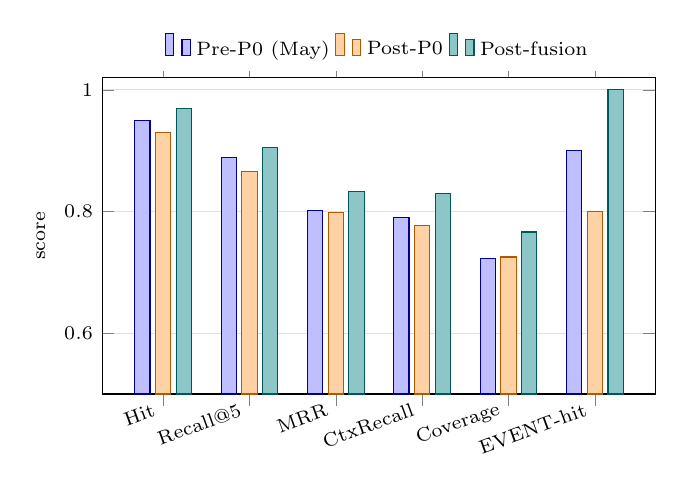
\begin{tikzpicture}
\begin{axis}[
  width=8.6cm, height=5.6cm,
  ybar, bar width=5.5pt,
  enlarge x limits=0.14,
  ymin=0.5, ymax=1.02,
  ylabel={score},
  symbolic x coords={Hit,Recall@5,MRR,CtxRecall,Coverage,EVENT-hit},
  xtick=data,
  x tick label style={font=\scriptsize, rotate=20, anchor=east},
  y tick label style={font=\scriptsize},
  ylabel style={font=\scriptsize},
  legend style={font=\scriptsize, at={(0.5,1.02)}, anchor=south,
                legend columns=3, draw=none},
  ymajorgrids, grid style={black!12},
]
\addplot+[fill=blue!25, draw=blue!60!black] coordinates
  {(Hit,0.950) (Recall@5,0.8892) (MRR,0.8020) (CtxRecall,0.7908)
   (Coverage,0.7223) (EVENT-hit,0.90)};
\addplot+[fill=orange!35, draw=orange!70!black] coordinates
  {(Hit,0.930) (Recall@5,0.8658) (MRR,0.7978) (CtxRecall,0.7767)
   (Coverage,0.7253) (EVENT-hit,0.80)};
\addplot+[fill=teal!45, draw=teal!70!black] coordinates
  {(Hit,0.970) (Recall@5,0.9058) (MRR,0.8335) (CtxRecall,0.8297)
   (Coverage,0.7664) (EVENT-hit,1.00)};
\legend{Pre-P0 (May), Post-P0, Post-fusion}
\end{axis}
\end{tikzpicture}
\caption{The three-round shape of the evidence chain: the KG
completeness overhaul alone (orange) reads flat-to-negative on a
head-entity benchmark; unlocking the ranking layer (teal) recovers and
surpasses every indicator.}
\label{fig:evolution}
\end{figure}

Table~\ref{tab:evolution} and Fig.~\ref{fig:evolution} give the
headline: hit rate 0.97, recall@5 0.906, context recall 0.830, coverage
0.766; EVENT hit rate 1.00 with context recall 0.728 --- not merely
recovering the P0 regression but surpassing the pre-P0 state on every
EVENT indicator; and the margin over the semantic baseline widened to
$+0.16$ hit rate / $+0.148$ recall@5. Four questions flipped
from miss to hit --- the two persistent pre-P0 failures (EVENT\_008 via
aliases$+$EQ, EVENT\_014 via curated node $+$ fusion) and the two TSK
casualties (EVENT\_017 via TSK declassing, EVENT\_019 via the
keyword-exact pin) --- and all five forensic cases of
Table~\ref{tab:tskforensic} recovered, with EVENT\_015 regaining full
recall (its Matthew and Luke anchors returned to the top-5). The quick retrieval loop and
the full pipeline agree bit-exactly on every retrieval metric.

Two residuals are instructive rather than problematic. GENERAL NDCG sits
$0.08$ below post-P0 --- traced per question to the \emph{retirement} of
pin-based artificial top-1 placement (the correct passages remain in
top-5; the earlier perfect MRR was pin manufactured, so the ``drop'' is
the removal of an artifact, not a regression). PERSON\_004 remains the
single PERSON miss, by design out of scope for ranking repairs
(Section~\ref{sec:diagnosis}).

\subsection{$\alpha$ Ablation: A Complementary Structure}
\label{sec:ablation}

Sweeping the fusion coefficient with everything else fixed
(Table~\ref{tab:ablation}) decomposes the remediation:

\begin{table}[!t]
\caption{$\alpha$ Ablation (Retrieval-Only Loop; All Other Repairs
Active)}
\label{tab:ablation}
\centering
\begin{threeparttable}
\begin{tabular}{@{}lcc@{}}
\toprule
 & $\alpha=0$ (pure reranker) & $\alpha=0.3$ (deployed) \\
\midrule
Overall hit rate & 0.97 & 0.97 \\
EVENT hit rate & 1.00 & 1.00 \\
EVENT recall@5 & baseline & $+0.025$ \\
TOPIC MRR & baseline & $+0.133$ \\
NDCG@5 & baseline & $-0.02$ \\
\bottomrule
\end{tabular}
\begin{tablenotes}\footnotesize
\item $\alpha=0$ keeps the data repairs, chunk remap, pin changes, and
keyword-exact pin; only the fusion term is disabled.
\end{tablenotes}
\end{threeparttable}
\end{table}

\begin{itemize}
\item \textbf{Discrete repairs saturate hit rate.} At $\alpha=0$, hit
rate is already 0.97 and EVENT already 1.00: curated data (aliases,
nodes) and the dictionary pin are responsible for \emph{whether} the
answer appears at all.
\item \textbf{Continuous fusion recovers the tail.} $\alpha=0.3$ adds
EVENT recall@5 $+0.025$ --- the multi-gospel parallel anchors of the
Last Supper carry $s_{\mathrm{rr}}\approx 0.01$--$0.02$ and only fusion
returns them --- and TOPIC MRR $+0.133$, at the cost of NDCG@5
$-0.02$ (high-prior, low-surface-form candidates advancing).
\item \textbf{The trade resolves by downstream use.} All top-5 passages
enter the generation context, so recall dominates internal ordering;
$\alpha=0.3$ was adopted.
\end{itemize}

The two mechanisms substitute for the reranker's surface-form monopoly
at \emph{different layers} --- discrete repairs at the
candidate/vocabulary layer, fusion at the scoring layer --- and their
effects are complementary rather than redundant. This
decomposition is the constructive counterpart of the negative result:
the same graph assets that read as zero in Section~\ref{sec:p0} produce
the Table~\ref{tab:evolution} gains once the ranking layer transmits
them.
